 % TODO: Liste prérequis actu pour les cours optionnels
% TODO: Explication des résultats d'examen
% TODO: Rôle de l'ICA

\documentclass[11pt,french]{article}
	%% Francisation de LaTeX
	\usepackage{babel}
	\usepackage[autolanguage]{numprint}
	\usepackage[utf8]{inputenc}
	\usepackage[T1]{fontenc}
	\usepackage{icomma}
	\usepackage[hidelinks]{hyperref}
	\usepackage{xcolor}
	\usepackage{graphicx}
  	\graphicspath{{./fig/}}
	\hypersetup{
    colorlinks,
    linkcolor={red!50!black},
    citecolor={blue!50!black},
    urlcolor={blue!80!black}}
    \usepackage{graphicx}
    \usepackage{tabularx}
    \usepackage{caption}
    \usepackage{wrapfig}
    \usepackage{enumitem}
    \usepackage{lipsum}  % generates filler text

\usepackage{fancyhdr}
\fancyhf{} % clear all header and footers
\renewcommand{\headrulewidth}{0pt} % remove the header rule
\rfoot{\thepage}
\pagestyle{fancy}

\usepackage{epigraph}
% \epigraphsize{\small}% Default
\setlength\epigraphwidth{8cm}
\setlength\epigraphrule{0pt}

\usepackage{etoolbox}

\makeatletter

\patchcmd{\epigraph}{\@epitext{#1}}{\itshape\@epitext{#1}}{}{}
\makeatother

\title{\vspace{2cm}
	   Guide pour les examens professionnels en actuariat
       \vspace{2cm}}
\author{\textbf{Auteur} \\
				Antoine Beaupré \vspace{2cm} \\
				\textbf{Coauteurs} \\
				David Beauchemin \\ 
				Kaesey-Andrew Lépine \\
				Matis Brassard-Verrier \vspace{4cm}}


\AtBeginDocument{\def\labelitemi{$\bullet$}}



\begin{document}
\pagenumbering{Roman}
\maketitle
\thispagestyle{fancy}

\newpage

\begin{abstract}
Ce guide s'adresse en premier lieu aux étudiants qui débutent dans le baccalauréat en actuariat, mais les plus expérimentés y trouveront tout de même de l'information pertinente. Plutôt que de décrire en long et en large le processus d'examens professionnels et les méthodes d'étude à préconiser, ce guide renvoie systématiquement le lecteur vers des pages web en fournissant une brève description de ce qu'on retrouvera à cette adresse.\footnote{Les opinions qui sont exprimées dans ce document n'impliquent en aucun cas l'École d'actuariat, la \emph{Society of Actuaries}, la \emph{Casualty Actuarial Society} ou n'importe quelle autre organisation. Ce document n'est pas non plus une source d'information officielle et devrait seulement être considéré comme un outil de référence.}{\tiny} 
\end{abstract}

\clearpage
\vspace*{\stretch{2}}
\begin{center}
\begin{minipage}{.6\textwidth}
\epigraph{We do not rise to the level of our expectations. We fall to the level of our training.}{--- \textup{Archiloque}, 712-664 av. J.-C.}
\end{minipage}
\end{center}
\vspace{\stretch{3}}
\clearpage

\newpage
\tableofcontents

\newpage
\pagenumbering{arabic}
\setcounter{page}{1}

%%%%%%%%%%%%% Content %%%%%%%%%%%%%%%%%%%%%%%%%%%%%%

\section*{Généralités}
\label{sec:generalites}
\addcontentsline{toc}{section}{Généralités}

\subsection*{Les examens professionnels}
\label{subsec:examsprofs}
\addcontentsline{toc}{subsection}{Les examens professionnels}
\captionsetup{justification=centering}
Bien souvent, les examens professionnels sont l'une des premières choses dont l'on entend parler lorsqu'il est question d'actuariat. Il y a beaucoup d'informations disponibles sur le sujet, autant à partir de sources officielles que sur différents forums de discussion.\vspace{\baselineskip}

Afin d'avoir une bonne idée du cheminement, je vous suggère de vous référer en premier lieu aux informations se trouvant sur les sites des deux principales organisations professionnelles en actuariat: la \href{https://soa.org/member/}{\emph{Society of Actuaries (SOA)}} et la \href{http://www.casact.org/}{\emph{Casualty Actuarial Society (CAS)}}. Essentiellement, ce sont leurs champs d'activité différents qui distinguent ces deux organisations:
\begin{itemize}
\item La CAS se spécialise dans l'assurance IARD (Incendie, accident et risques divers).
\item La SOA regroupe les branches assurance-vie, retraite, assurance-maladie, investissement et gestion de risques en entreprise.\footnote{ Il est à noter que la spécialisation \emph{General Insurance} de la SOA n'est pas reconnue par l'Institut canadien des actuaires (ICA).}
\end{itemize}
\vspace{\baselineskip}

Vous remarquerez qu'il y a, autant du côté de la CAS que de la SOA, une série d'examens préliminaires suivie par des examens avancés. Certains examens préliminaires sont communs à tous, peu importe la spécialisation que l'on désire atteindre. Ces examens sont P/1, FM/2 et IFM/3F. La raison pour laquelle il y a deux appellations par examen préliminaire est que la SOA et la CAS ne nomment pas de la même façon ces examens dans leur cheminement. Du côté de la SOA, on a les examens P, FM et IFM, alors que ces mêmes examens se nomment 1, 2 et 3F du côté de la CAS. La section \nameref{sec:prelims} du présent document parlera plus en détails du contenu de ces examens, du matériel d'étude à utiliser et des façons de bien s'y préparer.\vspace{\baselineskip}

Après ces examens communs aux deux sociétés, il y a d'autres examens préliminaires à accomplir, mais ces examens sont différents selon que l'on suive le chemin de la SOA ou de la CAS. Du côté de la SOA, il faut réussir les examens STAM, LTAM, SRM et PA. Quant à la CAS, elle exige la réussite des examens MAS-I, MAS-II, 5 et 6. Une fois ces examens préliminaires réussis et d'autres exigences satisfaites\footnote{Ces exigences supplémentaires sont des crédits VEE (voir la section \nameref{subsec:vee}), des modules d'apprentissage en ligne et des séminaires de professionnalisme. Les exigences supplémentaires de la SOA et de la CAS diffèrent sur plusieurs points.}, le candidat atteint le rang d'Associé (ASA ou ACAS selon la société choisie), qui est le but à moyen terme de la plupart des étudiants et des récents gradués en actuariat. \vspace{\baselineskip}

Une fois le titre d'Associé atteint, d'autres examens attendent ceux qui veulent aller plus loin. Ce sont les examens avancés, qui une fois réussis, permettent au candidat d'atteindre le titre de Fellow (FSA ou FCAS, encore une fois selon la société choisie). Vous aurez peut-être remarqué que même si la SOA regroupe plusieurs branches assez distinctes, elle offre les mêmes examens préliminaires à tous ses candidats. Ce sont donc plutôt les examens avancés qui permettent d'atteindre une spécialisation dans cette société. Pour ce qui est de la CAS, comme c'est une société qui est déjà spécialisée dans une seule branche, les examens avancés sont communs à tous. Le présent document ne traitera pas de chacun des examens avancés en détail, en raison du nombre très élevé d'examens différents et du fait que le document s'adresse surtout à des apprentis actuaires qui ont réussi peu ou pas d'examens. Toutefois, vous pouvez consulter la \nameref{subsec:faq} si les détails techniques de ces examens avancés vous intéressent. \vspace{\baselineskip}

Vous pouvez visualiser la progression nécessaire (examens préliminaires, autres exigences et examens avancés) jusqu'au titre de Fellow, autant pour la SOA que pour la CAS, dans la figure de la page suivante. \newpage

\begin{center}
\begin{figure}[hp]
\includegraphics[width=1\textwidth]{tableau_ICA.png}
\caption{Cheminement professionnel en actuariat --- Grille fournie par Joseph Gabriel de l'Institut canadien des actuaires}
\end{figure}
\par
\end{center}


Autre élément important à savoir: le 1er juillet 2018, les exigences à satisfaire pour devenir Associé de la SOA ont subi des changements importants. Le syllabus de la plupart des examens ont été modifiés, les exigences des VEE ont changé et deux examens complètement nouveaux ont été créés. Ces changements sont mentionnés pour chaque examen et VEE en question lorsqu'il est traité. Pour avoir plus d'informations sur les changements de juillet 2018 et pour connaître la réponse de la CAS à ces changements, vous pouvez consulter la sous-section \nameref{subsec:changeasa} du présent document. \vspace{\baselineskip}

Il y a énormément d'informations sur les sites de la SOA et de la CAS, mais ils ne disent pas tout non plus. La SOA parle souvent  d'une \emph{règle du pouce} d'environ 100 heures d'étude par heure d'examen, sans donner de détails vraiment sur la façon de répartir ces heures ou quel matériel d'étude utiliser par exemple. Les différents forums de discussion sont une excellente ressource pour connaître ce genre d'informations, les deux principaux étant \href{http://www.actuarialoutpost.com/}{\emph{Actuarial Outpost}} et \href{https://www.reddit.com/r/actuary}{\emph{/r/actuary}}. La page \href{https://www.reddit.com/r/actuary/wiki/index#wiki_the_frequently_asked_questions_.28faqs.29}{\emph{FAQ}} de \emph{/r/actuary} contient beaucoup d'informations utiles pour les gens qui débutent en actuariat. Également, la discussion \href{https://www.reddit.com/r/actuary/comments/1enzdd/how_long_to_get_to_asa_is_two_years_possible/}{\emph{How long to get to ASA}} de ce même site contient des réponses intéressantes au sujet du temps nécessaire pour compléter les examens. \vspace{\baselineskip}

Pour connaître des statistiques au sujet des examens professionnels, vous pouvez consulter le site \href{http://actuarial-lookup.com/}{\emph{actuarial-lookup}}. Ce site contient des données de 2007 jusqu'à aujourd'hui. \vspace{\baselineskip}

Vous trouverez les dates importantes pour les examens préliminaires sur cette \href{https://www.soa.org/Education/Exam-Req/Exam-Day-Info/edu-2018-cbt-test-schedule.aspx}{page}. J'en profite également pour mentionner qu'en vous inscrivant avec votre adresse courriel universitaire, vous serez éligible à un rabais étudiant pour les examens IFM/3F, STAM/4 et LTAM. Voir cette \href{https://soa.org/Education/Exam-Req/Syllabus-Study-Materials/Exam-and-Module-Fees.aspx}{page} pour plus de détails concernant les coûts d'inscription. \vspace{\baselineskip}

\newpage

\subsection*{L'ICA et les accréditations d'examens professionnels}
\label{subsec:ica}
\addcontentsline{toc}{subsection}{L'ICA et les accréditations d'examens professionnels}

Une autre organisation est d'une grande importance pour les étudiants canadiens en actuariat: il s'agit de \href{https://www.cia-ica.ca/fr/accueil}{l'Institut canadien des actuaires (ICA)}. Là où la SOA et la CAS gèrent plutôt l'aspect académique de la profession, l'ICA s'occupe surtout de l'aspect professionnel et du droit de pratique des actuaires canadiens. Il y a également des titres d'Associé et de Fellow de l'ICA (AICA et FICA), mais il ne faut pas réussir d'autres examens pour avoir ces titres; en effet, ils sont \textit{associés} aux titres d'Associé et de Fellow obtenus dans une autre société (SOA ou CAS). En d'autres mots, les étudiants en actuariat font des examens pour obtenir des titres de la SOA ou de la CAS, et une fois ces titres obtenus, les titres correspondants de l'ICA viennent automatiquement avec. \vspace{\baselineskip} 

Le tableau ci-dessous a pour but de clarifier les différences entre les rôles des trois organismes mentionnés jusqu'à présent.

\begin{center}
\begin{figure}[hp]
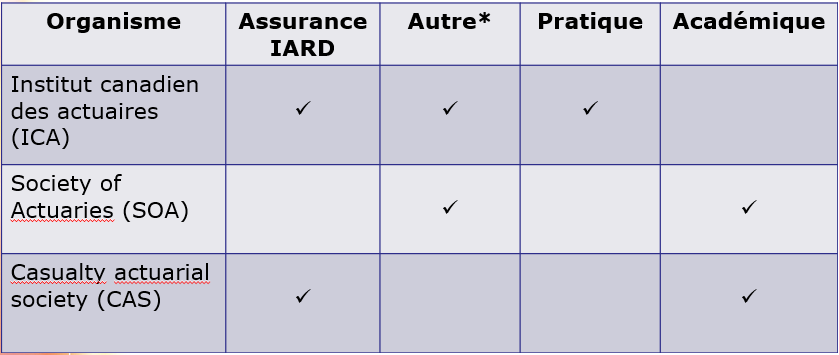
\includegraphics[width=1\textwidth]{roles_organismes.png}
\caption{Différences entre les rôles de la SOA, de la CAS et de l'ICA}
\end{figure}
\par
\end{center}

Il y a quelques années, l'ICA a lancé un programme d'accréditation des examens professionnels. Ce projet vise à valoriser davantage les connaissances apprises lors de l'éducation supérieure et à permettre aux étudiants de ne pas avoir à être testés deux fois sur les mêmes connaissances (une fois à l'école et une autre fois dans les examens professionnels). De fait, si un étudiant a des notes jugées adéquates à certains cours qui sont associés à un certain examen professionnel, alors l'étudiant peut se faire \textit{accréditer} l'examen professionnel et ne pas avoir du tout à le faire. Par contre, si les notes requises ne sont pas atteintes dans les cours en question, l'étudiant ne peut pas se faire accréditer l'examen professionnel et il doit le tenter et le réussir. \vspace{\baselineskip}

Vous trouverez l'information quant aux cours qui permettent d'obtenir les accréditations d'examen de l'ICA dans votre \href{https://www.act.ulaval.ca/programmes-et-cours/premier-cycle/guide-de-letudiant/}{guide de l'étudiant}. Cette information se trouve généralement dans les dernières pages du document. Remarquez que tous les examens préliminaires de la SOA sont accréditables, sauf le premier examen (\nameref{subsec:examp}). \vspace{\baselineskip}

Il est important de savoir que la CAS reconnaît les accréditations de l'ICA, mais que la SOA ne les reconnaît pas encore. Ainsi, un candidat qui obtient des accréditations pour certains examens peut obtenir les titres de Fellow de l'ICA et de la CAS mais, s'il est du côté de la SOA, il ne pourra pas devenir Fellow de la SOA --- il sera seulement Fellow de l'ICA. En théorie, cela ne devrait pas être grave puisque c'est l'ICA qui gère le droit de pratique au Canada et pas la SOA. Cependant, ce ne sont pas toutes les entreprises qui voient d'un bon œil le fait de s'être fait accréditer des examens professionnels et de ne pas avoir les titres de la SOA. La décision de prendre les accréditations d'examens ou non reste à la discrétion de chaque étudiant et je vous conseille de bien vous informer à ce sujet et de peser le pour et le contre selon votre avancement et vos intérêts.

\newpage

\subsection*{Les crédits VEE}
\label{subsec:vee}
\addcontentsline{toc}{subsection}{Les crédits VEE}
Les crédits VEE (\emph{Validation by Educational Experience}) sont une composante nécessaire pour obtenir le titre d'Associé. Les VEE permettent de couvrir des sujets qui ne sont pas formellement testés lors des examens préliminaires. La CAS et la SOA ont deux VEE en commun: le VEE \emph{Corporate Finance and Accounting} et le VEE \emph{Economics}. La SOA compte également le VEE \emph{Applied Statistical Methods}. Anciennement, la CAS comptait également ce troisième VEE, mais ils ont décidé de l'enlever suite à la création de l'Examen S (maintenant MAS-1).\vspace{\baselineskip}

Les crédits VEE peuvent être complétés en obtenant une note d'au moins B- dans certains cours du baccalauréat. Présentement, les cours qui permettent d'obtenir les VEE sont:
\begin{itemize}
\item Pour le VEE \emph{Applied Statistical Methods}, \textit{ACT-2000 Analyse statistique des risques actuariels}. Avant le 1er juillet 2018, c'étaient les cours \textit{ACT-2003 Modèles linéaires en actuariat} \textbf{et} \textit{ACT-2010 Séries chronologiques} qui procuraient le VEE.
\item Pour le VEE \emph{Economics}, \textit{ECN-1000 Principes de microéconomie} \textbf{et} \textit{ECN-1010 Principes de macroéconomie}. 
\item Pour le VEE \emph{Corporate Finance and Accounting}, \textit{ACT-1006 Gestion du risque financier I} \textbf{et} \textit{CTB-1000 Comptabilité générale}. La partie \emph{Accounting} du VEE sera nécessaire à partir du 1er juillet 2019. Également, la partie \emph{Corporate Finance} sera allégée à partir du 1er juillet 2019 (il faudra des cours de finance moins avancés pour obtenir le VEE à partir de cette date), car les éléments de finance plus avancés auront plutôt été distribués dans les différents examens professionnels. Remarquez que les changements de ce VEE seront effectifs à partir du 1er juillet 2019, et pas à partir du 1er juillet 2018 comme pour les autres VEE et examens.
\end{itemize}
\vspace{\baselineskip}

Comme vous pouvez le constater, les VEE ont subi plusieurs modifications suite aux changements des prérequis pour devenir Associé de juillet 2018. Pour ceux qui auraient des questions sur les transitions des cours qui procurent les VEE, n'hésitez pas à nous contacter. \vspace{\baselineskip}

Advenant le cas où vous n'auriez pas la cote minimale pour obtenir le crédit, vous devrez éventuellement compléter un cours en ligne sur le sujet du VEE en question, lequel sera suivi d'un examen.

\newpage

\subsection*{Alternatives et compléments aux manuels}
\label{subsec:alternatives}
\addcontentsline{toc}{subsection}{Alternatives et compléments aux manuels}
Il existe quelques alternatives et compléments aux manuels d'étude. Par exemple, les sites \href{http://www.theinfiniteactuary.com/}{\emph{The Infinite Actuary}} et \href{https://www.coachingactuaries.com/}{\emph{Coaching Actuaries}} offrent des formations préparatoires sous forme de vidéos pour tous les examens préliminaires (et certains examens avancés dans le cas de \emph{The Infinite Actuary}). Ces ressources sont toutefois peu populaires auprès des étudiants du baccalauréat, puisqu'elles sont souvent dispendieuses.\vspace{\baselineskip}

Un complément incontournable aux manuels d'étude est le système dynamique de génération d'examens ADAPT. Ce système est offert par le site \href{https://www.coachingactuaries.com/}{\emph{Coaching Actuaries}} et comporte une énorme banque de questions pour chacun des examens préliminaires. Le fonctionnement de ADAPT est plutôt simple; on débute au niveau 3, le système génère des examens pour vous et, dépendamment de votre résultat à l'examen, votre niveau (\emph{Earned Level} en anglais) va augmenter ou diminuer. Le niveau de l'examen correspond à sa difficulté; plus il est élevé, plus il sera difficile. Vous pourrez également plus facilement voir quelles sont les sections de l'examen où vous avez le plus de difficulté et créer des quiz spécifiquement sur ces sections afin de vous améliorer. L'objectif est d'atteindre un niveau 7 (sans tricher --- évidemment), puisque les statistiques disponibles montrent qu'environ 90\% des gens qui ont atteint ce niveau ont réussi leur examen. Vous aurez aussi droit à un rabais de 20\% pour les examens P, FM, IFM (MFE) grâce au code LAVALPC20 et un rabais de 30\% pour les examens C (STAM/MAS-2), MLC (LTAM), S (MAS-1) grâce au code LAVALPC30. Voir ce \href{https://www.youtube.com/watch?v=ZBxLa2J5jhs}{vidéo} pour une brève présentation de ADAPT. \vspace{\baselineskip}

L'association étudiante offre les manuels d'études P/1, FM/2, MFE/3 et S en version papier, ainsi que les livres pour les modules de la \textit{SOA} (\textit{FAP}). De plus, les manuels P/1, FM/2, MFE/3, C/4, S et MLC sont disponibles en version électronique sur le \href{https://drive.google.com/open?id=0B6kXivc6X9LISE1ydE41UnY3UDQ}{\textit{Google Drive}}. Également, prochainement les nouveaux livres d'étude seront disponibles pour les nouveaux examens et les nouvelles versions des examens.
\newpage
\section*{Les examens préliminaires (partie I) - Communs SOA et CAS}
\label{sec:prelims}
\addcontentsline{toc}{section}{Les examens préliminaires (partie I) - Communs SOA et CAS}

\subsection*{Examen P/1}
\label{subsec:examp}
\addcontentsline{toc}{subsection}{Examen P/1}
\href{https://www.soa.org/education/exam-req/edu-exam-p-detail.aspx}{L'examen P/1} (P pour \textit{Probability}) a pour objectif de développer les notions essentielles de la théorie des probabilités dans le contexte de l'actuariat. La matière de cet examen est traitée dans le cours \textit{ACT-1002 Analyse probabiliste des risques actuariels}. Après avoir complété ce cours, des étudiants ont rapporté avoir étudié \textbf{environ} 50 à 100 heures pour l'examen P/1. Pour consulter les objectifs spécifiques de l'examen ainsi que d'autres informations, voir le syllabus. Cet examen est d'une durée de 3 heures et comporte 30 questions à choix multiples (choix A, B, C, D, E). La SOA a publié \href{http://www.soa.org/Files/Edu/edu-exam-p-sample-quest.pdf}{326 questions} types pour cet examen, accompagnées du \href{http://www.soa.org/Files/Edu/edu-exam-p-sample-sol.pdf}{solutionnaire}.\vspace{\baselineskip}

À mon avis, le meilleur manuel d'étude pour l'examen P/1 est celui de ASM, écrit par Abraham Weishaus. Le site \href{http://www.theinfiniteactuary.com/exams/1}{The Infinite Actuary} offre gratuitement quatre examens pratiques qui sont à peu près du même niveau que le véritable examen. C'est donc une excellente pratique pour vous. Enfin, une inscription à \href{https://www.coachingactuaries.com/}{ADAPT} peut également vous permettre de mieux déterminer si vous êtes prêt à faire l'examen et donc s'avérer être un investissement très rentable.\vspace{\baselineskip}

Voici un exemple de plan d'étude pour l'examen P/1 (après avoir complété ACT-1002) :
\begin{enumerate}
\item Faire une lecture rapide du manuel ASM pour avoir une bonne vue d'ensemble de la matière à l'examen;
\item Relire les sections dans lesquelles vous avez plus de difficulté et faire des exercices jusqu'à devenir confortable;
\item Compléter les problèmes de la SOA en notant les problèmes que vous ne comprenez pas;
\item Relire les sections du manuel ASM pour combler les lacunes que vous aviez lorsque vous avez fait les problèmes de la SOA;
\item Débuter les examens pratiques dans le manuel ASM;
\item \textbf{Cinq jours avant l'examen :} faire deux examens par jour sur le site The Infinite Actuary;
\item \textbf{Trois jours avant l'examen :} refaire les problèmes que vous ne compreniez pas à l'étape trois et les problèmes ratés dans les examens pratiques;
\item \textbf{La journée avant l'examen :} faire une dernier survol léger de l'ensemble de la matière, relire ses notes et s'assurer de bien connaître les formules nécessaires.
\end{enumerate}
\vspace{\baselineskip}

Ce plan d'étude est seulement à titre indicatif et la majorité d'entre vous auront sans doute besoin de moins d'étude que ce qui y figure. Quelqu'un qui a bien réussi le cours ACT-1002 pourrait très bien faire une lecture rapide du manuel ASM, puis passer directement aux examens pratiques. Il faut garder en tête que les problèmes que vous devrez résoudre lors de l'examen P/1 seront moins compliqués que ceux du cours ACT-1002, mais la note de passage de cet examen est d'environ 70\% plutôt que d'être de 50\%. 

\newpage
\subsection*{Examen FM/2}
\label{subsec:examfm}
\addcontentsline{toc}{subsection}{Examen FM/2}
\href{https://www.soa.org/education/exam-req/edu-exam-fm-detail.aspx}{L'examen FM/2} (FM pour \textit{Financial Mathematics}) traite surtout des mathématiques financières et un peu des produits dérivés. Les cours du baccalauréat en actuariat en lien avec cet examen sont \textit{ACT-1001 Mathématiques financières} et \textit{ACT-2011 Gestion du risque financier II} pour la partie produits dérivés. Après avoir complété le cours \textit{ACT-1001 Mathématiques financières}, des étudiants ont rapporté avoir étudié \textbf{environ} 75 à 175 heures pour l'examen FM/2. Pour consulter les objectifs spécifiques de l'examen ainsi que d'autres informations, voir le syllabus. Cet examen est d'une durée de 3 heures et comporte 35 questions à choix multiples. La SOA a publié \href{https://www.soa.org/Files/Edu/2015/edu-2015-exam-fm-ques-theory.pdf}{133 questions} types sur les mathématiques financières ainsi que le \href{https://www.soa.org/Files/Edu/2015/edu-2015-exam-fm-sol-theory.pdf}{solutionnaire} et \href{https://www.soa.org/Files/Edu/edu-2014-10-exam-fm-ques.pdf}{64 questions} types sur les produits dérivés avec le \href{https://www.soa.org/Files/Edu/edu-2014-10-exam-fm-sol.pdf}{solutionnaire}.\vspace{\baselineskip} 

À mon avis, le meilleur manuel d'étude pour l'examen FM/2 est celui de ASM. Les explications sont extrêmement détaillées en plus d'avoir d'excellentes notes pour bien maîtriser la calculatrice BA II Plus, une compétence qui est très utile lors de l'examen. Personnellement, je n'avais pas utilisé ADAPT pour cet examen, puisque le manuel comporte déjà énormément de problèmes en plus d'examens pratiques qui sont comparables en difficulté au véritable examen. Vous trouverez, encore une fois, deux examens pratiques tout à fait gratuits sur le site \href{http://www.theinfiniteactuary.com/exams/2}{The Infinite Actuary}. La difficulté de ces deux examens pratiques est comparable au véritable examen.\vspace{\baselineskip} 

\textbf{Changements du curriculum de juillet 2018:} Le nouvel examen ressemblera beaucoup à celui en vigueur depuis juin 2017 (en effet, depuis cette date, les seules notions de produits dérivés évaluées pour l'examen FM sont les swaps de taux d'intérêt) à l'exception de certaines notions du VEE \textit{Corporate Finance} qui seront maintenant évaluées. Ainsi, l'essentiel de la matière qui se trouve à l'examen sera maintenant traitée dans les cours \textit{ACT-1001 Mathématiques financières} et \textit{ACT-2011 Gestion du risque financier I}. Je vous conseille de consulter le syllabus pour plus d'informations sur les notions traitées à l'examen.


\newpage
\subsection*{Examen IFM/3F (Anciennement MFE)}
\label{subsec:exammfe}
\addcontentsline{toc}{subsection}{Examen IFM/3F (Anciennement MFE)}
\href{https://www.soa.org/Education/Exam-Req/edu-exam-ifm-detail.aspx}{L'examen IFM/3F} (IFM pour \textit{Investment and Financial Markets}) traite de la base théorique de la finance corporative et des modèles financiers et de leurs applications dans des contextes d'assurance et de gestion de risques. Les notions de produits dérivés seront utilisées comme base. Le cours du baccalauréat en lien avec cet examen est \textit{ACT-2011 Gestion du risque financier II}. Pour consulter les objectifs spécifiques de l'examen ainsi que d'autres informations, voir le syllabus. Cet examen est d'une durée de 3 heures et comporte 30 questions à choix multiples. La SOA a publié \href{http://www.soa.org/files/edu/edu-exam-mfe-sample-quest-sol.pdf}{76 questions} types pour cet examen. Je vous conseille toutefois de ne pas trop perdre de temps sur ces questions, puisqu'elles ne sont pas représentatives de l'examen.\vspace{\baselineskip}

Pour ce qui est du manuel d'étude à utiliser, le plus populaire est celui de ASM, écrit par Abraham Weishaus. Toutefois, le \href{http://howardmahler.com/Teaching/MFE.html}{manuel} d'Howard Mahler est beaucoup apprécié par plusieurs et coûte seulement 50 USD en version électronique. Par contre, la principale critique au sujet de ce manuel est qu'il y a des lacunes au niveau des concepts plus avancés (mouvement brownien, lemme d'Itô, modèles pour les taux d'intérêt, etc.)\vspace{\baselineskip}

Pour cet examen, ADAPT est un outil extrêmement utile. Plusieurs personnes sur des forums de discussion disent que c'est probablement l'examen où les questions dans ADAPT sont le plus similaires aux questions lors du véritable examen. D'ailleurs, beaucoup d'étudiants rapportent qu'ils ont rencontré des questions dans l'examen formulées exactement de la même façon que des questions dans ADAPT. De plus, les examens pratiques du livre ASM ne sont pas tout à fait représentatifs du véritable examen et c'est pourquoi je recommande très fortement l'utilisation de ADAPT pour l'examen IFM/3F.\vspace{\baselineskip}

\textbf{Changements du curriculum de juillet 2018:} Comme c'était déjà le cas depuis juin 2017, les concepts plus poussés mathématiquement (mouvement brownien, processus stochastiques, modèles de taux d'intérêt) sont retirés du syllabus de cet examen et seront plutôt traités dans les examens avancés de Fellowship appropriés. Également, à partir de juillet 2018, certaines notions de finance corporative et de théorie moderne du portefeuille sont ajoutés au syllabus de l'examen IFM. Je vous conseille de consulter le syllabus pour plus d'informations sur les notions traitées à l'examen.


\newpage




\section*{Les examens préliminaires (partie II) - Côté SOA}
\label{sec:prelimssuitesoa}
\addcontentsline{toc}{section}{Les examens préliminaires (partie II) - Côté SOA}

\subsection*{Examen STAM (Anciennement C)}
\label{subsec:examstam}
\addcontentsline{toc}{subsection}{Examen STAM (Anciennement C)}
\href{https://www.soa.org/Education/Exam-Req/edu-exam-stam-detail.aspx}{L'examen STAM} (STAM pour \textit{Short-Term Actuarial Mathematics}) est une introduction à la modélisation, à l'analyse de données statistiques dans un contexte d'affaires, à l'estimation et à la création d'intervalles de confiance pour les décisions basées sur les modèles statistiques. Les cours du baccalauréat en lien avec cet examen sont \textit{ACT-2001 Introduction à l'actuariat II}, \textit{ACT-2005 Mathématiques actuarielles IARD I} et \textit{ACT-2008 Mathématiques actuarielles IARD II}. Pour consulter les objectifs spécifiques de l'examen ainsi que d'autres informations, voir le syllabus. Cet examen est d'une durée de 3h30 et comporte 35 questions à choix multiples. La SOA a publié \href{http://www.soa.org/files/edu/edu-exam-c-sample-quest.pdf}{305 questions} types pour cet examen, accompagnées du \href{http://www.soa.org/files/edu/edu-exam-c-sample-sol.pdf}{solutionnaire}.\vspace{\baselineskip}

Pour ce qui est du manuel d'étude à utiliser, il y a principalement deux écoles de pensée qui s'affrontent. Le manuel le plus populaire est probablement celui de ASM, encore une fois écrit par Abraham Weishaus. Par contre, certaines personnes estiment que les explications sont souvent trop peu détaillées et qu'il est donc difficile de bien comprendre la matière avec ce manuel. À l'opposé, les gens qui utilisent le \href{http://howardmahler.com/Teaching/C.html}{manuel} d'Howard Mahler disent que l'auteur prend le temps de bien expliquer toute la théorie et qu'il présente un bon nombre d'astuces qui aident à gagner en rapidité au moment de l'examen. Le seul problème, c'est que le manuel de Mahler fait 5528 pages, contre 1282 pages pour le livre ASM (en excluant les examens pratiques --- il n'y a pas d'examens pratiques dans le livre de Mahler, ils doivent être achetés séparément). \vspace{\baselineskip}

Malgré tout, pour ceux qui ont déjà suivi les cours du baccalauréat qui traitent de la matière à l'examen STAM/4, le manuel ASM est sans doute suffisamment détaillé pour que vous atteigniez un niveau de préparation adéquat. Pour ceux qui voudraient faire l'examen avant de suivre les cours de mathématiques actuarielles IARD, je conseille d'utiliser le livre de Mahler.\vspace{\baselineskip}

Pour ce qui est des examens pratiques, plusieurs personnes sur les forums de discussion ont de très bons commentaires pour ceux d'\href{http://howardmahler.com/Teaching/C.html}{Howard Mahler}, vendus séparément de son livre. Bien qu'ils semblent généralement être considérés comme difficiles, ces examens pratiques permettent vraiment de bien appliquer la matière et d'établir des connexions entre les différents sujets. À l'opposé, plusieurs ont tendance à dire que ADAPT n'est pas un bon outil pour cet examen, puisque la formulation des questions n'est pas représentative du véritable examen. \vspace{\baselineskip}

\textbf{Changements du curriculum de juillet 2018:} Parmi tous les examens déjà existants, l'ancien examen C est celui qui a subi le plus gros changement avec les nouvelles exigences de juillet 2018. Le matériel statistique de base qui était auparavant dans le syllabus de l'examen C est maintenant évalué dans le VEE \textit{Mathematical Statistics}. Par conséquent, les connaissances de ce VEE sont maintenant considérées comme prérequises à l'examen, bien qu'elles ne soient pas évaluées dans ce dernier. De plus, le matériel traitant de tables de mortalités est maintenant évalué dans l'exam LTAM. Ces sujets sont remplacés par des notions de produits d'assurance court terme (entre autres, assurance santé, assurance habitation et assurance responsabilité). Des notions de tarification et de méthodes de réserves pour les contrats d'assurance court terme sont égalements ajoutées au syllabus. Je vous conseille de consulter ce dernier pour plus d'informations sur les notions traitées à l'examen. \vspace{\baselineskip}

\newpage


\subsection*{Examen LTAM (Anciennement MLC)}
\label{subsec:examltam}
\addcontentsline{toc}{subsection}{Examen LTAM (Anciennement MLC)}

\href{https://www.soa.org/Education/Exam-Req/edu-exam-ltam-detail.aspx}{L'examen LTAM} (LTAM pour \textit{Long-Term Actuarial Mathematics}) évalue les connaissances théoriques sur les modèles de paiements contingents (des engagements à long terme auxquels sont associés des flux monétaires qui peuvent se produire ou non), de même que l'application de ces modèles à l'assurance et à divers risques financiers.  Les cours du baccalauréat en lien avec cet examen sont \textit{ACT-2004 Mathématiques actuarielles vie I}, \textit{ACT-2007 Mathématiques actuarielles vie II} et \textit{ACT-4106 Modèles avancés en assurance de personnes}. Pour consulter les objectifs spécifiques de l'examen ainsi que d'autres informations, voir le syllabus. Cet examen est d'une durée de 4 heures et le nombre de questions n'est pas encore annoncé. \vspace{\baselineskip}

Contrairement aux autres examens préliminaires de la SOA, l'examen LTAM ne peut pas être fait dans un centre Prometric; on doit absolument le faire en version papier. Cette différence est expliquée par le fait que l'examen LTAM est le seul examen préliminaire à contenir non seulement des questions à choix multiples, mais aussi des questions à développement, ce qui le rapproche d'une certaine manière aux examens avancés. Une autre différence notable est que l'examen LTAM est le seul examen préliminaire auquel on peut avoir accès aux examens des sessions précédentes. Vous pouvez les trouver sur \href{https://www.soa.org/education/exam-req/syllabus-study-materials/edu-multiple-choice-exam.aspx}{cette page} (cherchez les examens MLC, qui correspondent à l'ancien nom de l'examen LTAM). Il va donc de soit que les examens précédents sont une ressource essentielle pour ceux qui comptent se préparer à passer cet examen. En plus de ces examens précédents, la SOA a aussi publié \href{http://www.soa.org/files/edu/edu-2014-spring-mlc-ques.pdf}{322 questions types à choix multiples} (accompagnées de leur \href{http://www.soa.org/files/edu/edu-2014-spring-mlc-sol.pdf}{solutionnaire}), ainsi que \href{http://www.soa.org/files/edu/edu-2014-spring-mlc-ques-sol.pdf}{22 questions types à développement} (les questions et leurs solutions sont comprises dans le document). \vspace{\baselineskip}

Au sujet des manuels d'étude, le plus populaire au sein des étudiants du baccalauréat semble être le manuel ASM, rédigé par Abraham Weishaus. Les commentaires sur ce manuel de 1927 pages sont assez bons, et la majorité des gens s'entendent pour dire qu'il couvre bien toute la matière du syllabus de l'examen. Par contre, certaines personnes ont comme avis que le manuel ASM passe trop rapidement sur certains concepts, ou bien présente parfois des raccourcis, voire même du par coeur, sans miser totalement sur la compréhension globale de la matière. Ceux qui préfèreraient apprendre avec une compréhension plus globale de la matière et qui ne voient pas de problème à dépenser un certain montant peuvent se tourner vers le cours en ligne de \href{http://www.theinfiniteactuary.com/exams/45}{\textit{The Infinite Actuary}} ou celui de \href{https://www.coachingactuaries.com/ltam/}{\textit{Coaching Actuaries}}. Ces cours présentent la matière en vidéos d'une manière que plusieurs trouvent dynamique et motivante. Ces cours en ligne possèdent aussi des solutions à des centaines d'exercices ainsi que plusieurs examens pratiques. \vspace{\baselineskip}

Les ressources les plus populaires demeurent néanmoins le manuel ASM accompagné des questions types et des anciens examens de la SOA. Un conseil qui revient souvent de ceux qui ont fait l'examen est de ne pas négliger les questions à développement, car c'est souvent là que les personnes moins préparées manquent de temps à l'examen. \vspace{\baselineskip}

Pour ce qui est d'ADAPT, certains trouvent que c'est une ressource utile pour cet examen, mais d'autres affirment qu'ADAPT reprend beaucoup de questions déjà publiées par la SOA, que ce soient des questions types ou des questions tirées des anciens examens. Certains estiment donc qu'ADAPT n'est pas un investissement nécessaire pour l'examen LTAM si l'on a les questions types et les anciens examens en notre possession, mais le choix reste le vôtre. \vspace{\baselineskip}

\textbf{Changements du curriculum de juillet 2018:} Certaines notions de l'ancien examen MLC sont retirées, comme les courbes de rendement et les notions portant sur le risque diversifiable. C'est aussi le cas de l'assurance vie universelle, qui est maintenant vue lors des modules FAP. Également, certains sujets qui étaient originellement au syllabus de l'examen C sont maintenant évalués dans cet examen, de même que des notions supplémentaires sur les produits d'assurance vie et de rentes. Je vous conseille de consulter le syllabus pour plus d'informations sur les notions traitées à l'examen. \vspace{\baselineskip} \newpage




\subsection*{Examen SRM}
\label{subsec:examsrm}
\addcontentsline{toc}{subsection}{Examen SRM}

\href{https://www.soa.org/Education/Exam-Req/edu-exam-srm-detail.aspx}{L'examen SRM} (SRM pour \textit{Statistics for Risk Modeling}) est un examen totalement nouveau du côté de la SOA. Cet examen a été instauré lors des changements aux prérequis pour devenir Associé de juillet 2018. La SOA, en sondant les employeurs et les institutions académiques, a conclu que les aspirants actuaires devaient démontrer des compétences en analyse prédictive qui vont plus loin que les simples notions académiques de régression linéaire et de séries chronologiques qui étaient testées avant juillet 2018. Il a été décidé que ces nouvelles compétences en analyse prédictive seraient d'abord évaluées de manière classique lors de l'examen SRM, puis de manière plus pratique dans \href{https://www.soa.org/Education/Exam-Req/edu-exam-pa-detail.aspx}{l'examen PA} (voir la section suivante). Il est également à noter que les connaissances du VEE \textit{Mathematical Statistics} sont jugées comme prérequises à cet examen. \vspace{\baselineskip}

L'examen SRM teste des connaissances en modèles linéaires, en séries chronologiques, en arbres de décision, en partitionnement de données et en analyse en composantes principales. Les candidats doivent également être en mesure de choisir et de valider des modèles statistiques. Les cours du baccalauréat en lien avec cet examen sont, entre autres, \textit{ACT-2003 Modèles linéaires en actuariat} et \textit{ACT-2010 Séries chronologiques}. Pour consulter les objectifs spécifiques de l'examen ainsi que d'autres informations, voir le syllabus. Cet examen est d'une durée de 3 heures 30 et comporte 35 questions à choix multiples. La première séance de l'examen SRM se tiendra en septembre 2018. \vspace{\baselineskip}



\subsection*{Examen PA}
\label{subsec:exampa}
\addcontentsline{toc}{subsection}{Examen PA}

\href{https://www.soa.org/Education/Exam-Req/edu-exam-pa-detail.aspx}{L'examen PA} (PA pour \textit{Predictive Analytics}) est également un examen totalement nouveau du côté de la SOA. Cet examen a été instauré lors des changements aux prérequis pour devenir Associé de juillet 2018. Il se démarque des autres examens en ce qu'il n'utilise pas la même méthode que les examens précédents pour tester la connaissance d'objectifs d'apprentissage. Maintenant que les nouvelles compétences en analyse prédictive ont été testées de manière classique lors de \href{https://www.soa.org/Education/Exam-Req/edu-exam-srm-detail.aspx}{l'examen SRM} (voir la section précédente), elles le sont maintenant de manière plus pratique dans cet examen PA. Il est donc obligatoire d'avoir fait et réussi l'examen SRM (ou bien d'avoir un crédit de transition pour cet examen) avant de pouvoir s'inscrire à l'examen PA. \vspace{\baselineskip}

On peut affirmer que l'examen PA est séparé en 2 parties:
\begin{enumerate}
\item La première partie consiste en des modules d'apprentissage en ligne qui ont pour seul but de préparer à la deuxième partie. Ces modules poussent plus loin les notions apprises pour l'examen SRM et clarifient les attentes de la SOA au sujet de la deuxième partie.
\item La deuxième partie consiste en la réalisation pratique d'un rapport. Les candidats se font présenter un jeu de données et un problème corporatif jugé réaliste. Les candidats ont 5 heures pour préparer un rapport qui présente leur solution à ce problème.
\end{enumerate}
\vspace{\baselineskip}

L'examen se déroule dans un centre Prometric, et les candidats travaillent sur un ordinateur où ils peuvent utiliser les programmes Excel, Word et RStudio. À la fin des 5 heures, les candidats doivent remettre un rapport et tout le code R et les autres éléments qui peuvent supporter la solution qu'ils ont présentée dans leur rapport. La première séance de l'examen PA se tiendra en décembre 2018. De par sa nature, l'examen ne sera pas corrigé comme les examens préliminaires qui le précèdent, mais plutôt selon \href{https://www.soa.org/Education/General-Info/edu-guide-written-exams-seminar-vids.aspx}{la méthode utilisée pour corriger les examens avancés de Fellowship}.

\newpage

\section*{Les examens préliminaires (partie II) - Côté CAS}
\label{sec:prelimssuitecas}
\addcontentsline{toc}{section}{Les examens préliminaires (partie II) - Côté CAS}

Cette section est encore en développement. \vspace{\baselineskip}


\subsection*{Examen MAS-I (Anciennement S)}
\label{subsec:examMAS_I}
\addcontentsline{toc}{subsection}{Examen MAS-I (Anciennement S)}

\href{http://www.casact.org/admissions/syllabus/index.cfm?fa=MASI&parentID=391}{L'examen MAS-I} (MAS-I pour \textit{Modern Actuarial Statistics-I}) est une introduction aux modèles probabilistes (les processus stochastiques et les modèles de survie), à l'utilisation des tests statistiques, aux modèles linéaires et aux séries chronologiques. Les cours du baccalauréat en lien avec cet examen sont \textit{ACT-2009 Processus stochastiques}, \textit{ACT-2003 Modèles linéaires en actuariat} et \textit{ACT-2010 Séries chronologiques}. Pour consulter les objectifs spécifiques de l'examen ainsi que d'autres informations, voir le syllabus. Cet examen est d'une durée de 4 heures et devrait comporter 40 questions à choix multiples à correction négative comme l'ancien examen S. La CAS a publié des anciens \href{http://www.casact.org/admissions/studytools/examS/}{examens} types du S, ainsi que quelques \href{http://www.casact.org/admissions/studytools/examS/Sample_Questions.pdf}{questions} de l'examen S.\vspace{\baselineskip}

Pour ce qui est du manuel d'étude à utiliser, il y a le manuel d'\href{https://drive.google.com/open?id=0B6kXivc6X9LISGhkVUkzLW5sSnc}{ASM}, encore une fois écrit par Abraham Weishaus. Par contre, certaines personnes estiment que les \href{https://drive.google.com/open?id=0B6kXivc6X9LIOUs3SDF3NmVKNGM}{examens pratiques} d'Howard Mahler sont très similaires aux examens et donc plus adéquats pour l'étude. Par contre, avec les changements, la situation pourrait changer. \vspace{\baselineskip}


\subsection*{Examen MAS-II (Anciennement C)}
\label{subsec:examMAS_II}
\addcontentsline{toc}{subsection}{Examen MAS-II (Anciennement C)}

\href{http://www.casact.org/admissions/syllabus/index.cfm?fa=MASII&parentID=392}{L'examen MAS-II} (MAS-II pour \textit{Modern Actuarial Statistics-II}) est une introduction à la modélisation, à l'analyse de données statistiques dans un contexte d'affaires, à la crédibilité, à l'estimation et à la création d'intervalles de confiance pour les décisions basées sur les modèles statistiques. Les cours du baccalauréat en lien avec cet examen sont \textit{ACT-2001 Introduction à l'actuariat II}, \textit{ACT-2005 Mathématiques actuarielles IARD I} et \textit{ACT-2008 Mathématiques actuarielles IARD II}. Pour consulter les objectifs spécifiques de l'examen ainsi que d'autres informations, voir le syllabus. Cet examen est d'une durée de 4h00 à correction négative et le nombre de questions n'est pas encore annoncé. La SOA a publié \href{http://www.soa.org/files/edu/edu-exam-c-sample-quest.pdf}{305 questions} types pour cet examen, accompagnées du \href{http://www.soa.org/files/edu/edu-exam-c-sample-sol.pdf}{solutionnaire}. Il s'agit du matériel d'étude du C, du nouveau matériel d'étude sera disponible d'ici là.\vspace{\baselineskip}

Pour ce qui est du manuel d'étude et des examens formatifs à utiliser, le matériel devrait être similaire à l'ancien C (soit le manuel de ASM, encore une fois écrit par Abraham Weishaus et le \href{http://howardmahler.com/Teaching/C.html}{manuel} d'Howard Mahler). Plus d'information sera ajoutée avec les développements des changements.\vspace{\baselineskip}

\subsection*{Examen 5}
\label{subsec:exam5}
\addcontentsline{toc}{subsection}{Examen 5}

Sous-section en développement. \vspace{\baselineskip}


\subsection*{Examen 6}
\label{subsec:exam6}
\addcontentsline{toc}{subsection}{Examen 6}

Sous-section en développement. \vspace{\baselineskip}


\newpage

\section*{Autres informations}
\label{sec:autres}
\addcontentsline{toc}{section}{Autres informations}

\subsection*{Liens utiles}
\label{subsec:liens}
\addcontentsline{toc}{subsection}{Liens utiles}
Pour ceux qui sont intéressés par le domaine de la finance ou qui cherchent à étendre leurs champs d'expertise, la désignation professionnelle CFA peut être une très bonne option. C'est sans doute la désignation du monde de la finance qui est la plus reconnue à l'international et un nombre considérable d'actuaires la possèdent. Afin d'obtenir cette désignation, l'on doit passer trois examens (\emph{Level I, II} et \emph{Level III}) et avoir quatre ans d'expérience pertinente dans le milieu de la finance. Concernant l'expérience demandée, il est difficile de connaître les critères exactes du CFA Institute mais, généralement, il faut qu'une majorité du temps de travail de ces quatre années soit relié à la gestion d'actifs au sens large. Les examens \emph{Level II \emph{et} Level III} sont offerts seulement une fois par année, le premier samedi du mois de juin, alors que le \emph{Level I} est également offert au mois de décembre. Pour plus d'informations, consulter la page du \href{https://www.cfainstitute.org/Pages/index.aspx}{\emph{CFA Institute}}. Vous pouvez également lire l'article \href{http://blog.coachingactuaries.com/why-would-actuaries-consider-getting-a-cfa/}{\emph{Why would Actuaries consider getting a CFA?}}.\vspace{\baselineskip}

%%% TODO: faire des sections qui décrivent les examens CFA? De plus en plus de gens qui s'intéressent au titre...

Ceux qui sont intéressés par l'informatique et le \emph{data science} pourront s'informer au sujet de la création du \href{http://www.casact.org/press/index.cfm?fa=viewArticle&articleID=3083}{CAS Institute}.\vspace{\baselineskip} 


\newpage
\subsection*{Changements aux prérequis pour devenir Associé}
\label{subsec:changeasa}
\addcontentsline{toc}{subsection}{Changements aux prérequis pour devenir Associé}
\subsubsection*{SOA}
La SOA a amorcé en 2017 un important processus de restructuration des prérequis pour devenir Associé. La nouvelle structure est effective à partir du $1^{er}$ juillet 2018. Le plus gros changement est l’ajout de deux nouveaux examens (SRM et PA), mais ce sont quasi toutes les composantes qui sont modifiées d'une manière ou d'une autre. Ces changements au curriculum sont guidés par deux facteurs clés:

\begin{itemize}
\item L'ajout de l'analyse prédictive aux connaissances jugées essentielles pour devenir Associé;
\item Un meilleur équilibre entre les notions d'assurance court terme et long terme.
\end{itemize}
 Les changements subis par chaque composante sont mentionnés dans la section qui lui correspond.

\subsubsection*{CAS}
De son côté, la CAS a aussi amorcé un processus de restructuration pour 2018, mais les changements sont moins drastiques que pour la SOA. En pratique, l'ancien examen S devient l'examen MAS-I, et l'ancien examen C devient l'examen MAS-II. Également, la CAS a annoncé qu’elle reconnaîtrait les nouveaux formats des examens FM/2 et IFM/3F instaurés par la SOA. \textit{Les changements seront traités plus en détail dans les sections correspondantes du document dans une prochaine version de celui-ci.}

\vspace{\baselineskip} 

Quelques liens supplémentaires :
\begin{enumerate}
\item \href{https://www.soa.org/Education/General-Info/2016-asa-cera-curriculum-changes.aspx}{Annonce du 28 juin par la SOA}
\item \href{https://soa.qualtrics.com/CP/File.php?F=F_0TDd9bj143TrCW9}{Annonce préliminaire de la SOA (janvier 2016)}
\item \href{https://www.soa.org/Education/General-Info/2016-transition-rules-asa-candidated.aspx}{L’équivalence des examens actuels dans le système à venir}
\item \href{http://www.casact.org/press/index.cfm?fa=viewArticle&articleID=3273}{Annonce de la CAS pour le nouveau format de FM/2 et MFE/3F}
\end{enumerate}
\vspace{\baselineskip} 

Les diagrammes ci-dessous vous permettent d'observer d'une manière graphique les changements apportés aux prérequis pour devenir Associé, tant du côté de la SOA que de celui de la CAS.

\begin{figure}[hp]
\begin{center}
\textbf{Changements aux prérequis pour devenir Associé (SOA)}\par\medskip
\end{center}
\hfill\includegraphics[scale=0.8]{Change_ASA.PNG}\hspace*{\fill}
\caption{Équivalences des examens actuels dans le système à venir (SOA)}
\end{figure}
\par
\begin{figure}[hp]
\begin{center}
\textbf{Changements aux prérequis pour devenir Associé (CAS)}\par\medskip
\end{center}
\hfill\includegraphics[scale=0.6]{Change_ASA_CAS.PNG}\hspace*{\fill}
\caption{Équivalences des examens actuels dans le système à venir (CAS)}
\end{figure}
\par

\newpage

%%%%%%%%%%%%% Annexes %%%%%%%%%%%%%%%%%%%%%%%%%%%%%%
\section*{Annexes}
\label{sec:annexes}
\addcontentsline{toc}{section}{Annexes}

\subsection*{Procédure pour l'inscription aux examens préliminaires}
\label{subsec:inscriptionexams}
\addcontentsline{toc}{subsection}{Procédure pour l'inscription aux examens préliminaires}
La procédure pour l'inscription aux examens préliminaires est la même pour les candidats de la CAS et les candidats de la SOA. Elle comporte principalement deux étapes : l'inscription à l'examen sur le site de la SOA et fixer la date sur le site de Prometric.\footnote{Cette dernière étape est omise si vous faites l'examen papier.}\vspace{\baselineskip} 

\begin{enumerate}
\item \textbf{Inscription à l'examen sur le site de la SOA}
\begin{itemize}
\item Se rendre sur la \href{https://www.soa.org/Education/Exam-Req/Registration/edu-registration.aspx}{page d'inscription}. 
\item Sélectionner l'examen de votre choix. Si ce n'est pas déjà fait, vous devrez vous créer un compte sur le site de la SOA.
\item Payer le montant indiqué.
\item Vous recevrez une lettre de confirmation de votre commande par courriel, qui contient notamment votre numéro de candidat.
\end{itemize}\vspace{\baselineskip}

\item \textbf{Fixer la date sur le site de Prometric}
\begin{itemize}
\item Vous recevrez un deuxième courriel (\textit{Letter of confirmation}) qui vous informera de vous inscrire sur le site de Prometric. Ce courriel est envoyé environ 3 à 5 jours ouvrables après avoir payé pour l'examen.
\item Suivre les instructions qui figurent dans ce courriel afin de fixer une date pour votre examen. Pour ce faire, vous devrez utiliser votre numéro d'éligibilité qui figure dans ce second courriel.
\end{itemize}
\end{enumerate}

\newpage


\subsection*{Procédure pour réclamer les crédits VEE (SOA et CAS)}
\label{subsec:reclamvee}
\addcontentsline{toc}{subsection}{Procédure pour réclamer les crédits VEE (SOA et CAS)}
Une fois que vous avez complété le ou les cours nécessaires pour obtenir votre crédit VEE, vous devez faire la demande pour que celui-ci soit ajouté à votre dossier.\footnote{Vous pouvez trouver des informations concernant les cours et les cotes qui permettent d'obtenir les crédits VEE dans votre \href{https://www.act.ulaval.ca/programmes-et-cours/premier-cycle/guide-de-letudiant/}{guide étudiant} ou encore sur cette \href{https://soa.org/Education/Exam-Req/Instructions-for-VEE-Directory.aspx}{page de la SOA}.} Un autre point important à savoir est qu'il faut avoir réussi au moins 2 examens professionnels avant de pouvoir réclamer des VEE. Il n'y a aucune limite de temps pour réclamer des VEE: si le cours réussi correspond aux exigences de la SOA au moment où vous réussi le cours \textbf{ou} en ce moment, vous pouvez réclamer le VEE correspondant, peu importe à quel moment le cours a été réussi.\vspace{\baselineskip} 

La procédure est la même pour les candidats de la SOA et les candidats de la CAS. Elle comporte principalement deux étapes: remplir le formulaire en ligne de la SOA et acheminer le relevé de notes de l'Université Laval au bureau d'administration des VEE de la SOA.\vspace{\baselineskip} 

\begin{enumerate}
\item \textbf{Remplir le formulaire de la SOA}
\begin{itemize}
\item Se rendre sur la \href{https://soa.org/education/exam-req/edu-vee.aspx}{page d'information sur les VEE}. 
\item Cliquer sur le type d'application en ligne pour le VEE qui vous intéresse (\textit{Apply for VEE Economics Credit}, \textit{Apply for VEE Accounting and Finance Credit} ou \textit{Apply for VEE Mathematical Statistics Credit}).
\item Entrer vos informations personnelles et cliquer sur \textit{Select School / University} pour pouvoir accéder à la liste de cours qui sont approuvés pour les VEE.
\item Sélectionner le pays et la province, puis sélectionner l'Université Laval. La liste de cours devrait apparaître. 
\item Cibler la ligne du cours que vous avez complété et entrer la cote obtenue et la date à laquelle vous avez terminé ce cours. 
\item Cliquer sur \textit{Select} (complètement à gauche de la ligne). Il vous reste ensuite simplement à payer le montant qui sera indiqué. En ce moment, le montant est de 50\$ US par VEE réclamé.
\end{itemize}\vspace{\baselineskip} \newpage
\item \textbf{Acheminer le relevé de notes de l'Université Laval à la SOA}
\begin{itemize}
\item Se rendre sur la \href{https://www.reg.ulaval.ca/cms/DemDoc/releveNotes}{page du Bureau du registraire pour les relevés de notes}.
\item Remplir le formulaire \textbf{REG-910-RN}. Le relevé de notes doit être acheminé au bureau d'administration des VEE de la SOA. L'adresse se trouve sur cette \href{https://soa.org/education/exam-req/course-info/edu-vee-applying-process.aspx}{page}.
\item Acheminer ce formulaire au bureau du registraire en suivant les indications sur la page concernant les relevés de notes. Des frais de 9\$ sont à prévoir pour la production du relevé de notes officiel.
\end{itemize}
\end{enumerate}

\newpage

\subsection*{Procédure pour réclamer une accréditation d'examen professionnel de l'ICA}
\label{subsec:reclamaccredit}
\addcontentsline{toc}{subsection}{Procédure pour réclamer une accréditation d'examen professionnel de l'ICA}

La procédure pour réclamer des accréditations de l'ICA est similaire sur certains points à la procédure pour réclamer des crédits VEE. Si vous avez eu les notes suffisantes dans certains cours pour pouvoir réclamer des accréditations\footnote{Vous pouvez trouver des informations concernant les cours et les cotes qui permettent d'obtenir les accréditations dans votre \href{https://www.act.ulaval.ca/programmes-et-cours/premier-cycle/guide-de-letudiant/}{guide étudiant}.}, vous avez trois ans pour suivre la procédure suivante, qui comporte principalement deux étapes: remplir le formulaire de l'ICA et l'acheminer au bureau de l'ICA avec un relevé de notes de l'Université Laval.\vspace{\baselineskip} 

\begin{enumerate}
\item \textbf{Remplir le formulaire de l'ICA}
\begin{itemize}
\item Se rendre sur la \href{http://www.cia-ica.ca/fr/adhesion/programme-d-agr\%C3\%A9ment-universitaire-(pau)-de-l-ica---page-d'accueil/renseignements-pour-les-candidats}{page d'information sur les accréditations d'examens}. 
\item Imprimer et remplir à la main le formulaire de demande disponible sur la page.
\item En ce moment, les frais demandés sont de 75\$ CAD par accréditation réclamée. Vous pouvez régler ces frais en ligne, par téléphone ou en joignant un chèque à votre formulaire; les informations pertinentes à ce sujet sont exposées dans le formulaire.
\end{itemize}\vspace{\baselineskip}
\item \textbf{Acheminer le formulaire et un relevé de notes officiel à l'ICA}
\begin{itemize}
\item Le but est d'avoir en votre possession votre relevé de notes officiel de l'université Laval et de le joindre vous-même au formulaire de l'ICA. Pour ce faire, vous pouvez simplement vous présenter au Bureau du registraire et demander la production d'un relevé de notes officiel (et par le fait même, ne pas avoir à remplir de formulaire).
\item Si vous ne pouvez pas vous rendre physiquement au Bureau du registraire, se rendre sur la \href{https://www.reg.ulaval.ca/cms/DemDoc/releveNotes}{page du Bureau du registraire pour les relevés de notes} et remplir le formulaire \textbf{REG-910-RN}. Désignez-vous comme destinataire, ce qui vous permettra de recevoir votre relevé chez vous. Acheminer ce formulaire au bureau du registraire en suivant les indications sur la page concernant les relevés de notes. 
\item Des frais de 9\$ sont à prévoir pour la production du relevé de notes officiel, que ça soit sur place ou avec l'envoi d'un formulaire.
\item Maintenant que vous avez le relevé de notes officiel en votre possession, il est très important de ne pas ouvrir l'enveloppe, ce qui briserait le sceau officiel du registraire et causerait le refus de votre demande.
\item Acheminer le formulaire de l'ICA, le relevé de notes officiel et le chèque (si vous payez par chèque) au bureau de l'ICA à Ottawa. L'adresse se trouve sur le formulaire de demande de l'ICA.
\end{itemize}
\end{enumerate}

\newpage



%%%%%%%%%%%%% FAQ %%%%%%%%%%%%%%%%%%%%%%%%%%%%%%
\subsection*{Foire aux questions}
\label{subsec:faq}
\addcontentsline{toc}{subsection}{Foire aux questions}
Cette section est en construction. Envoyez-moi vos questions par rapport aux examens professionnels, au cheminement en actuariat ou sur tout autre sujet que vous jugerez pertinent et je mettrai à jour cette section du document avec les réponses à vos questions. Vous pouvez rejoindre les auteurs aux adresses courriels suivantes: \emph{antoine.beaupre.1@ulaval.ca}, \emph{david.beauchemin.5@ulaval.ca}, \emph{kaesey-andrew.lepine.1@ulaval.ca} et \emph{matis.brassard-verrier.1@ulaval.ca}.\newline

\begin{itemize}
\item \textbf{Que faut-il faire exactement pour passer du statut d’associé à celui de fellow, autant du côté de la SOA que de la CAS? Y a-t-il des critères spécifiques ou bien est-ce plutôt flou, etc.}
	\begin{itemize}
	\item Pour ceux qui désirent se spécialiser en assurance IARD, il faut compléter trois autres examens de la CAS $-$ les examens 7, 8 et 9 $-$ pour atteindre le titre FCAS une fois que l'on est ACAS. Il s'agit tous d'examens de 4h. Pour plus de détails, voir la \href{http://www.casact.org/admissions/process/}{charte} des examens (elle n'inclut pas les changements de juillet 2018). 
	\item Pour ce qui est de la SOA, il y a quatre modules et trois examens avancés (deux de cinq heures, un de deux ou quatre heures) pour atteindre le titre de FSA une fois que l'on est ASA. Ces examens sont spécialisés et l'on doit donc choisir la branche qui nous intéresse, voir \href{https://www.soa.org/Education/Exam-Req/edu-fsa-req.aspx}{ici} pour plus de détail.
	\end{itemize}
\item \textbf{En général, quel est le coût pour appliquer à un examen professionnel? (préliminaires ou spécialisés)}
	\begin{itemize}
	\item Les coûts pour un examen préliminaire sont environ entre 200 et 300 \$ US en incluant les rabais étudiants. Tous les coûts sont décrits disponible sur le site de la \href{https://www.soa.org/Education/Exam-Req/Syllabus-Study-Materials/Exam-and-Module-Fees.aspx}{SOA} et de la \href{http://www.casact.org/admissions/exams/}{CAS}.
	\end{itemize}
	\item \textbf{Quelle est la procédure des examens professionnels, se font-ils en ligne ou sur papier?}
	\begin{itemize}
	\item Les examens préliminaires s'offrent pour la plupart sur ordinateur et papier. On peut le faire papier à l'université, mais si l'on désire le faire sur ordinateur $-$ et avoir un résultat instantané $-$ il faut généralement se déplacer dans un centre Prometric à Montréal. À certains moments durant l'année (souvent en octobre et en mars), certains examens sont offerts sur ordinateur à Québec. Toutes les dates des examens papier et sur ordinateur sont disponibles sur les sites respectifs de la \href{https://www.soa.org/Education/Exam-Req/Exam-Day-Info/edu-2017-cbt-test-schedule.aspx}{SOA} et la \href{http://www.casact.org/admissions/exams/}{CAS}.
	\end{itemize}
\end{itemize}


\end{document}